\documentclass[twoside]{book}

% Packages required by doxygen
\usepackage{fixltx2e}
\usepackage{calc}
\usepackage{doxygen}
\usepackage[export]{adjustbox} % also loads graphicx
\usepackage{graphicx}
\usepackage[utf8]{inputenc}
\usepackage{makeidx}
\usepackage{multicol}
\usepackage{multirow}
\PassOptionsToPackage{warn}{textcomp}
\usepackage{textcomp}
\usepackage[nointegrals]{wasysym}
\usepackage[table]{xcolor}

% Font selection
\usepackage[T1]{fontenc}
\usepackage[scaled=.90]{helvet}
\usepackage{courier}
\usepackage{amssymb}
\usepackage{sectsty}
\renewcommand{\familydefault}{\sfdefault}
\allsectionsfont{%
  \fontseries{bc}\selectfont%
  \color{darkgray}%
}
\renewcommand{\DoxyLabelFont}{%
  \fontseries{bc}\selectfont%
  \color{darkgray}%
}
\newcommand{\+}{\discretionary{\mbox{\scriptsize$\hookleftarrow$}}{}{}}

% Page & text layout
\usepackage{geometry}
\geometry{%
  a4paper,%
  top=2.5cm,%
  bottom=2.5cm,%
  left=2.5cm,%
  right=2.5cm%
}
\tolerance=750
\hfuzz=15pt
\hbadness=750
\setlength{\emergencystretch}{15pt}
\setlength{\parindent}{0cm}
\setlength{\parskip}{3ex plus 2ex minus 2ex}
\makeatletter
\renewcommand{\paragraph}{%
  \@startsection{paragraph}{4}{0ex}{-1.0ex}{1.0ex}{%
    \normalfont\normalsize\bfseries\SS@parafont%
  }%
}
\renewcommand{\subparagraph}{%
  \@startsection{subparagraph}{5}{0ex}{-1.0ex}{1.0ex}{%
    \normalfont\normalsize\bfseries\SS@subparafont%
  }%
}
\makeatother

% Headers & footers
\usepackage{fancyhdr}
\pagestyle{fancyplain}
\fancyhead[LE]{\fancyplain{}{\bfseries\thepage}}
\fancyhead[CE]{\fancyplain{}{}}
\fancyhead[RE]{\fancyplain{}{\bfseries\leftmark}}
\fancyhead[LO]{\fancyplain{}{\bfseries\rightmark}}
\fancyhead[CO]{\fancyplain{}{}}
\fancyhead[RO]{\fancyplain{}{\bfseries\thepage}}
\fancyfoot[LE]{\fancyplain{}{}}
\fancyfoot[CE]{\fancyplain{}{}}
\fancyfoot[RE]{\fancyplain{}{\bfseries\scriptsize Generated by Doxygen }}
\fancyfoot[LO]{\fancyplain{}{\bfseries\scriptsize Generated by Doxygen }}
\fancyfoot[CO]{\fancyplain{}{}}
\fancyfoot[RO]{\fancyplain{}{}}
\renewcommand{\footrulewidth}{0.4pt}
\renewcommand{\chaptermark}[1]{%
  \markboth{#1}{}%
}
\renewcommand{\sectionmark}[1]{%
  \markright{\thesection\ #1}%
}

% Indices & bibliography
\usepackage{natbib}
\usepackage[titles]{tocloft}
\setcounter{tocdepth}{3}
\setcounter{secnumdepth}{5}
\makeindex

% Hyperlinks (required, but should be loaded last)
\usepackage{ifpdf}
\ifpdf
  \usepackage[pdftex,pagebackref=true]{hyperref}
\else
  \usepackage[ps2pdf,pagebackref=true]{hyperref}
\fi
\hypersetup{%
  colorlinks=true,%
  linkcolor=blue,%
  citecolor=blue,%
  unicode%
}

% Custom commands
\newcommand{\clearemptydoublepage}{%
  \newpage{\pagestyle{empty}\cleardoublepage}%
}

\usepackage{caption}
\captionsetup{labelsep=space,justification=centering,font={bf},singlelinecheck=off,skip=4pt,position=top}

%===== C O N T E N T S =====

\begin{document}

% Titlepage & ToC
\hypersetup{pageanchor=false,
             bookmarksnumbered=true,
             pdfencoding=unicode
            }
\pagenumbering{alph}
\begin{titlepage}
\vspace*{7cm}
\begin{center}%
{\Large Advanced Programming Final Project }\\
\vspace*{1cm}
{\large Generated by Doxygen 1.8.13}\\
\end{center}
\end{titlepage}
\clearemptydoublepage
\pagenumbering{roman}
\tableofcontents
\clearemptydoublepage
\pagenumbering{arabic}
\hypersetup{pageanchor=true}

%--- Begin generated contents ---
\chapter{Hierarchical Index}
\section{Class Hierarchy}
This inheritance list is sorted roughly, but not completely, alphabetically\+:\begin{DoxyCompactList}
\item \contentsline{section}{B\+ST$<$ K, V, C $>$}{\pageref{classBST}}{}
\item iterator\begin{DoxyCompactList}
\item \contentsline{section}{B\+ST$<$ K, V, C $>$\+:\+:Iterator$<$ K, V, C $>$}{\pageref{classBST_1_1Iterator}}{}
\begin{DoxyCompactList}
\item \contentsline{section}{B\+ST$<$ K, V, C $>$\+:\+:Const\+Iterator$<$ K, V, C $>$}{\pageref{classBST_1_1ConstIterator}}{}
\end{DoxyCompactList}
\end{DoxyCompactList}
\end{DoxyCompactList}

\chapter{Class Index}
\section{Class List}
Here are the classes, structs, unions and interfaces with brief descriptions\+:\begin{DoxyCompactList}
\item\contentsline{section}{\hyperlink{classBST}{B\+S\+T$<$ K, V, C $>$} \\*This class implements a simple Binary Search Tree }{\pageref{classBST}}{}
\item\contentsline{section}{\hyperlink{classBST_1_1ConstIterator}{B\+S\+T$<$ K, V, C $>$\+::\+Const\+Iterator$<$ K, V, C $>$} }{\pageref{classBST_1_1ConstIterator}}{}
\item\contentsline{section}{\hyperlink{classBST_1_1Iterator}{B\+S\+T$<$ K, V, C $>$\+::\+Iterator$<$ K, V, C $>$} }{\pageref{classBST_1_1Iterator}}{}
\end{DoxyCompactList}

\chapter{File Index}
\section{File List}
Here is a list of all documented files with brief descriptions\+:\begin{DoxyCompactList}
\item\contentsline{section}{\hyperlink{BST_8h}{B\+S\+T.\+h} \\*Header file for our Advanced Programming final project }{\pageref{BST_8h}}{}
\end{DoxyCompactList}

\chapter{Class Documentation}
\hypertarget{classBST}{}\section{B\+ST$<$ K, V, C $>$ Class Template Reference}
\label{classBST}\index{B\+S\+T$<$ K, V, C $>$@{B\+S\+T$<$ K, V, C $>$}}


This class implements a simple Binary Search Tree.  




{\ttfamily \#include $<$B\+S\+T.\+h$>$}

\subsection*{Classes}
\begin{DoxyCompactItemize}
\item 
class \hyperlink{classBST_1_1ConstIterator}{Const\+Iterator}
\item 
class \hyperlink{classBST_1_1Iterator}{Iterator}
\end{DoxyCompactItemize}
\subsection*{Public Member Functions}
\begin{DoxyCompactItemize}
\item 
\hyperlink{classBST_a3cba9e816367006087a999b5e1027d72}{B\+ST} ()
\item 
\hyperlink{classBST_a77d30398500d92fe8a906c72677eaafb}{$\sim$\+B\+ST} ()
\item 
\hyperlink{classBST}{B\+ST}$<$ K, V, C $>$ \& \hyperlink{classBST_a59e6c0bc7ce4ad71686ae26ca3f71d77}{operator=} (const \hyperlink{classBST}{B\+ST}$<$ K, V, C $>$ \&rhs)
\begin{DoxyCompactList}\small\item\em Copy assignment. \end{DoxyCompactList}\item 
\hyperlink{classBST_a447d9506675de51dbf56403fa2b910e8}{B\+ST} (const \hyperlink{classBST}{B\+ST}$<$ K, V, C $>$ \&rhs)
\begin{DoxyCompactList}\small\item\em Copy costructor. \end{DoxyCompactList}\item 
\hyperlink{classBST_af590b11504c8725c0c0b983ccda10517}{B\+ST} (\hyperlink{classBST}{B\+ST}$<$ K, V, C $>$ \&\&rhs)
\begin{DoxyCompactList}\small\item\em Move costructor. \end{DoxyCompactList}\item 
\hyperlink{classBST}{B\+ST}$<$ K, V, C $>$ \& \hyperlink{classBST_a487925834a1291eec64d6efac4fb9fab}{operator=} (const \hyperlink{classBST}{B\+ST} \&\&rhs)
\begin{DoxyCompactList}\small\item\em Move assignment. \end{DoxyCompactList}\item 
\mbox{\Hypertarget{classBST_a28d4d73ccb420ad1e0dbd36bc5252d74}\label{classBST_a28d4d73ccb420ad1e0dbd36bc5252d74}} 
\hyperlink{classBST_1_1Iterator}{Iterator} \hyperlink{classBST_a28d4d73ccb420ad1e0dbd36bc5252d74}{begin} ()
\begin{DoxyCompactList}\small\item\em Returns an \hyperlink{classBST_1_1Iterator}{Iterator} to the first in order node of the tree. \end{DoxyCompactList}\item 
\mbox{\Hypertarget{classBST_a7b050d8cffe441618e074e09139db869}\label{classBST_a7b050d8cffe441618e074e09139db869}} 
\hyperlink{classBST_1_1Iterator}{Iterator} \hyperlink{classBST_a7b050d8cffe441618e074e09139db869}{end} ()
\begin{DoxyCompactList}\small\item\em Returns a pointer to the end of the tree, indicated by nullptr. \end{DoxyCompactList}\item 
\mbox{\Hypertarget{classBST_ad8c1af62e5b5e0b119179f177633836e}\label{classBST_ad8c1af62e5b5e0b119179f177633836e}} 
\hyperlink{classBST_1_1ConstIterator}{Const\+Iterator} \hyperlink{classBST_ad8c1af62e5b5e0b119179f177633836e}{begin} () const
\begin{DoxyCompactList}\small\item\em Returns a const iterator to the first node. \end{DoxyCompactList}\item 
\mbox{\Hypertarget{classBST_a1901ddfeb7c806d46ed363c115049363}\label{classBST_a1901ddfeb7c806d46ed363c115049363}} 
\hyperlink{classBST_1_1ConstIterator}{Const\+Iterator} \hyperlink{classBST_a1901ddfeb7c806d46ed363c115049363}{end} () const
\begin{DoxyCompactList}\small\item\em Returns a const iterator to the last node. \end{DoxyCompactList}\item 
\mbox{\Hypertarget{classBST_a2ca4a971ca3c6239c78a167fff42afe5}\label{classBST_a2ca4a971ca3c6239c78a167fff42afe5}} 
\hyperlink{classBST_1_1ConstIterator}{Const\+Iterator} {\bfseries cbegin} () const
\item 
\mbox{\Hypertarget{classBST_a44b8111ddbf10213f1cf97946cf8cccd}\label{classBST_a44b8111ddbf10213f1cf97946cf8cccd}} 
\hyperlink{classBST_1_1ConstIterator}{Const\+Iterator} {\bfseries cend} () const
\item 
\hyperlink{classBST_1_1ConstIterator}{Const\+Iterator} \hyperlink{classBST_a78994b2b2383be06e93f2f3882bbc7e6}{find} (const K \&item) const
\begin{DoxyCompactList}\small\item\em Givena key value, it returns an \hyperlink{classBST_1_1Iterator}{Iterator} to a node in the tree. \end{DoxyCompactList}\item 
bool \hyperlink{classBST_ac149123e8192d8f8d29eee828c3ee74a}{insert} (const std\+::pair$<$ K, V $>$ \&pair)
\begin{DoxyCompactList}\small\item\em Inserts a new node in the tree. \end{DoxyCompactList}\item 
std\+::vector$<$ std\+::pair$<$ K, V $>$ $>$ \hyperlink{classBST_a1f96234b9a71bdb4c2edd88b0ef80743}{from\+B\+S\+Tto\+Vector} ()
\begin{DoxyCompactList}\small\item\em Auxiliary function used in the balance function. \end{DoxyCompactList}\item 
void \hyperlink{classBST_abdb2fbf5e98852e77cf2d576d6944795}{from\+Vectorto\+Balance} (const std\+::vector$<$ std\+::pair$<$ K, V $>$$>$ \&nodi, int primo, int ultimo)
\begin{DoxyCompactList}\small\item\em Auxiliary function used in the balance routine. \end{DoxyCompactList}\item 
\mbox{\Hypertarget{classBST_a06274e4538ebbf7630058aa2da577ffe}\label{classBST_a06274e4538ebbf7630058aa2da577ffe}} 
void \hyperlink{classBST_a06274e4538ebbf7630058aa2da577ffe}{balance} ()
\begin{DoxyCompactList}\small\item\em Creates a balanced \hyperlink{classBST}{B\+ST} starting from an unbalanced one. \end{DoxyCompactList}\item 
void \hyperlink{classBST_ab126433ade0fa5711341d80cd6a498ff}{clear} ()
\item 
void \hyperlink{classBST_ae7caa3e87e5840631ecd016dcddca593}{copy} (const std\+::unique\+\_\+ptr$<$ Node $>$ \&curr\+\_\+node)
\begin{DoxyCompactList}\small\item\em Supplementary function used to create a deep copy of a tree. \end{DoxyCompactList}\item 
\mbox{\Hypertarget{classBST_af4fdcab3a5e76bc3f1b75241caae4f99}\label{classBST_af4fdcab3a5e76bc3f1b75241caae4f99}} 
\hyperlink{classBST_1_1Iterator}{Iterator} \hyperlink{classBST_af4fdcab3a5e76bc3f1b75241caae4f99}{find} (const K \&key)
\begin{DoxyCompactList}\small\item\em non const version of the find function \end{DoxyCompactList}\end{DoxyCompactItemize}
\subsection*{Friends}
\begin{DoxyCompactItemize}
\item 
{\footnotesize template$<$class oK , class oV , class oC $>$ }\\std\+::ostream \& \hyperlink{classBST_abf0033be2689fd4cfbeee149b114536b}{operator$<$$<$} (std\+::ostream \&, const \hyperlink{classBST}{B\+ST}$<$ oK, oV, oC $>$ \&)
\begin{DoxyCompactList}\small\item\em Overload of the operator $<$$<$. \end{DoxyCompactList}\end{DoxyCompactItemize}


\subsection{Detailed Description}
\subsubsection*{template$<$class K, class V, class C = std\+::greater$<$\+K$>$$>$\newline
class B\+S\+T$<$ K, V, C $>$}

This class implements a simple Binary Search Tree. 


\begin{DoxyTemplParams}{Template Parameters}
{\em K} & is the typename of the key \\
\hline
{\em V} & is the typename of the value \\
\hline
{\em C} & is the typename of the operator used to compare different keys \\
\hline
\end{DoxyTemplParams}


\subsection{Constructor \& Destructor Documentation}
\mbox{\Hypertarget{classBST_a3cba9e816367006087a999b5e1027d72}\label{classBST_a3cba9e816367006087a999b5e1027d72}} 
\index{B\+ST@{B\+ST}!B\+ST@{B\+ST}}
\index{B\+ST@{B\+ST}!B\+ST@{B\+ST}}
\subsubsection{\texorpdfstring{B\+S\+T()}{BST()}\hspace{0.1cm}{\footnotesize\ttfamily [1/3]}}
{\footnotesize\ttfamily template$<$class K, class V, class C = std\+::greater$<$\+K$>$$>$ \\
\hyperlink{classBST}{B\+ST}$<$ K, V, C $>$\+::\hyperlink{classBST}{B\+ST} (\begin{DoxyParamCaption}{ }\end{DoxyParamCaption})\hspace{0.3cm}{\ttfamily [inline]}}

constructor of a new \hyperlink{classBST}{B\+ST} object \mbox{\Hypertarget{classBST_a77d30398500d92fe8a906c72677eaafb}\label{classBST_a77d30398500d92fe8a906c72677eaafb}} 
\index{B\+ST@{B\+ST}!````~B\+ST@{$\sim$\+B\+ST}}
\index{````~B\+ST@{$\sim$\+B\+ST}!B\+ST@{B\+ST}}
\subsubsection{\texorpdfstring{$\sim$\+B\+S\+T()}{~BST()}}
{\footnotesize\ttfamily template$<$class K, class V, class C = std\+::greater$<$\+K$>$$>$ \\
\hyperlink{classBST}{B\+ST}$<$ K, V, C $>$\+::$\sim$\hyperlink{classBST}{B\+ST} (\begin{DoxyParamCaption}{ }\end{DoxyParamCaption})\hspace{0.3cm}{\ttfamily [inline]}}

default destructor \mbox{\Hypertarget{classBST_a447d9506675de51dbf56403fa2b910e8}\label{classBST_a447d9506675de51dbf56403fa2b910e8}} 
\index{B\+ST@{B\+ST}!B\+ST@{B\+ST}}
\index{B\+ST@{B\+ST}!B\+ST@{B\+ST}}
\subsubsection{\texorpdfstring{B\+S\+T()}{BST()}\hspace{0.1cm}{\footnotesize\ttfamily [2/3]}}
{\footnotesize\ttfamily template$<$class K, class V, class C = std\+::greater$<$\+K$>$$>$ \\
\hyperlink{classBST}{B\+ST}$<$ K, V, C $>$\+::\hyperlink{classBST}{B\+ST} (\begin{DoxyParamCaption}\item[{const \hyperlink{classBST}{B\+ST}$<$ K, V, C $>$ \&}]{rhs }\end{DoxyParamCaption})\hspace{0.3cm}{\ttfamily [inline]}}



Copy costructor. 


\begin{DoxyParams}{Parameters}
{\em rhs} & the tree that we want to use for initialization \\
\hline
\end{DoxyParams}
\mbox{\Hypertarget{classBST_af590b11504c8725c0c0b983ccda10517}\label{classBST_af590b11504c8725c0c0b983ccda10517}} 
\index{B\+ST@{B\+ST}!B\+ST@{B\+ST}}
\index{B\+ST@{B\+ST}!B\+ST@{B\+ST}}
\subsubsection{\texorpdfstring{B\+S\+T()}{BST()}\hspace{0.1cm}{\footnotesize\ttfamily [3/3]}}
{\footnotesize\ttfamily template$<$class K, class V, class C = std\+::greater$<$\+K$>$$>$ \\
\hyperlink{classBST}{B\+ST}$<$ K, V, C $>$\+::\hyperlink{classBST}{B\+ST} (\begin{DoxyParamCaption}\item[{\hyperlink{classBST}{B\+ST}$<$ K, V, C $>$ \&\&}]{rhs }\end{DoxyParamCaption})\hspace{0.3cm}{\ttfamily [inline]}}



Move costructor. 


\begin{DoxyParams}{Parameters}
{\em rhs} & the tree that we need to move \\
\hline
\end{DoxyParams}


\subsection{Member Function Documentation}
\mbox{\Hypertarget{classBST_ab126433ade0fa5711341d80cd6a498ff}\label{classBST_ab126433ade0fa5711341d80cd6a498ff}} 
\index{B\+ST@{B\+ST}!clear@{clear}}
\index{clear@{clear}!B\+ST@{B\+ST}}
\subsubsection{\texorpdfstring{clear()}{clear()}}
{\footnotesize\ttfamily template$<$class K, class V, class C = std\+::greater$<$\+K$>$$>$ \\
void \hyperlink{classBST}{B\+ST}$<$ K, V, C $>$\+::clear (\begin{DoxyParamCaption}{ }\end{DoxyParamCaption})\hspace{0.3cm}{\ttfamily [inline]}}

Clears the current content of a given \hyperlink{classBST}{B\+ST} object \mbox{\Hypertarget{classBST_ae7caa3e87e5840631ecd016dcddca593}\label{classBST_ae7caa3e87e5840631ecd016dcddca593}} 
\index{B\+ST@{B\+ST}!copy@{copy}}
\index{copy@{copy}!B\+ST@{B\+ST}}
\subsubsection{\texorpdfstring{copy()}{copy()}}
{\footnotesize\ttfamily template$<$class K , class V , class C $>$ \\
void \hyperlink{classBST}{B\+ST}$<$ K, V, C $>$\+::copy (\begin{DoxyParamCaption}\item[{const std\+::unique\+\_\+ptr$<$ Node $>$ \&}]{curr\+\_\+node }\end{DoxyParamCaption})}



Supplementary function used to create a deep copy of a tree. 

This function is called by both the copy constructor and the copy assignemnt functions. To perform a deep copy we add a node with the same value as the one of the current node to a tree and then, if children are present, we call the the function on the children of the current node


\begin{DoxyParams}{Parameters}
{\em curr\+\_\+node} & a pointer to the current node \\
\hline
\end{DoxyParams}
\mbox{\Hypertarget{classBST_a78994b2b2383be06e93f2f3882bbc7e6}\label{classBST_a78994b2b2383be06e93f2f3882bbc7e6}} 
\index{B\+ST@{B\+ST}!find@{find}}
\index{find@{find}!B\+ST@{B\+ST}}
\subsubsection{\texorpdfstring{find()}{find()}}
{\footnotesize\ttfamily template$<$class K, class V, class C = std\+::greater$<$\+K$>$$>$ \\
\hyperlink{classBST_1_1ConstIterator}{Const\+Iterator} \hyperlink{classBST}{B\+ST}$<$ K, V, C $>$\+::find (\begin{DoxyParamCaption}\item[{const K \&}]{item }\end{DoxyParamCaption}) const}



Givena key value, it returns an \hyperlink{classBST_1_1Iterator}{Iterator} to a node in the tree. 


\begin{DoxyParams}{Parameters}
{\em item} & the key value that we want to look up \\
\hline
\end{DoxyParams}
\mbox{\Hypertarget{classBST_a1f96234b9a71bdb4c2edd88b0ef80743}\label{classBST_a1f96234b9a71bdb4c2edd88b0ef80743}} 
\index{B\+ST@{B\+ST}!from\+B\+S\+Tto\+Vector@{from\+B\+S\+Tto\+Vector}}
\index{from\+B\+S\+Tto\+Vector@{from\+B\+S\+Tto\+Vector}!B\+ST@{B\+ST}}
\subsubsection{\texorpdfstring{from\+B\+S\+Tto\+Vector()}{fromBSTtoVector()}}
{\footnotesize\ttfamily template$<$class K , class V , class C $>$ \\
std\+::vector$<$ std\+::pair$<$ K, V $>$ $>$ \hyperlink{classBST}{B\+ST}$<$ K, V, C $>$\+::from\+B\+S\+Tto\+Vector (\begin{DoxyParamCaption}{ }\end{DoxyParamCaption})}



Auxiliary function used in the balance function. 

Given a \hyperlink{classBST}{B\+ST} object the function returns a vector of pairs key-\/value in order. \mbox{\Hypertarget{classBST_abdb2fbf5e98852e77cf2d576d6944795}\label{classBST_abdb2fbf5e98852e77cf2d576d6944795}} 
\index{B\+ST@{B\+ST}!from\+Vectorto\+Balance@{from\+Vectorto\+Balance}}
\index{from\+Vectorto\+Balance@{from\+Vectorto\+Balance}!B\+ST@{B\+ST}}
\subsubsection{\texorpdfstring{from\+Vectorto\+Balance()}{fromVectortoBalance()}}
{\footnotesize\ttfamily template$<$class K , class V , class C $>$ \\
void \hyperlink{classBST}{B\+ST}$<$ K, V, C $>$\+::from\+Vectorto\+Balance (\begin{DoxyParamCaption}\item[{const std\+::vector$<$ std\+::pair$<$ K, V $>$$>$ \&}]{nodi,  }\item[{int}]{primo,  }\item[{int}]{ultimo }\end{DoxyParamCaption})}



Auxiliary function used in the balance routine. 

It creates a \hyperlink{classBST}{B\+ST} starting from an ordered vector. It starts by setting the middle element of the vector as root and then calls the function recursevly on the left and right halves of the vector


\begin{DoxyParams}{Parameters}
{\em nodi} & is the ordered pairs vector \\
\hline
{\em primo} & the index of the first element \\
\hline
{\em ultimo} & the index of the last element \\
\hline
\end{DoxyParams}
\mbox{\Hypertarget{classBST_ac149123e8192d8f8d29eee828c3ee74a}\label{classBST_ac149123e8192d8f8d29eee828c3ee74a}} 
\index{B\+ST@{B\+ST}!insert@{insert}}
\index{insert@{insert}!B\+ST@{B\+ST}}
\subsubsection{\texorpdfstring{insert()}{insert()}}
{\footnotesize\ttfamily template$<$class K , class V , class C $>$ \\
bool \hyperlink{classBST}{B\+ST}$<$ K, V, C $>$\+::insert (\begin{DoxyParamCaption}\item[{const std\+::pair$<$ K, V $>$ \&}]{pair }\end{DoxyParamCaption})}



Inserts a new node in the tree. 

If the node is the first one to be inserted it is set as the root of the tree.


\begin{DoxyParams}{Parameters}
{\em pair} & the key-\/value pair that we want to insert in our tree \\
\hline
\end{DoxyParams}
\mbox{\Hypertarget{classBST_a59e6c0bc7ce4ad71686ae26ca3f71d77}\label{classBST_a59e6c0bc7ce4ad71686ae26ca3f71d77}} 
\index{B\+ST@{B\+ST}!operator=@{operator=}}
\index{operator=@{operator=}!B\+ST@{B\+ST}}
\subsubsection{\texorpdfstring{operator=()}{operator=()}\hspace{0.1cm}{\footnotesize\ttfamily [1/2]}}
{\footnotesize\ttfamily template$<$class K, class V, class C = std\+::greater$<$\+K$>$$>$ \\
\hyperlink{classBST}{B\+ST}$<$K,V,C$>$\& \hyperlink{classBST}{B\+ST}$<$ K, V, C $>$\+::operator= (\begin{DoxyParamCaption}\item[{const \hyperlink{classBST}{B\+ST}$<$ K, V, C $>$ \&}]{rhs }\end{DoxyParamCaption})\hspace{0.3cm}{\ttfamily [inline]}}



Copy assignment. 


\begin{DoxyParams}{Parameters}
{\em rhs} & the tree that we want to copy from \\
\hline
\end{DoxyParams}
\mbox{\Hypertarget{classBST_a487925834a1291eec64d6efac4fb9fab}\label{classBST_a487925834a1291eec64d6efac4fb9fab}} 
\index{B\+ST@{B\+ST}!operator=@{operator=}}
\index{operator=@{operator=}!B\+ST@{B\+ST}}
\subsubsection{\texorpdfstring{operator=()}{operator=()}\hspace{0.1cm}{\footnotesize\ttfamily [2/2]}}
{\footnotesize\ttfamily template$<$class K, class V, class C = std\+::greater$<$\+K$>$$>$ \\
\hyperlink{classBST}{B\+ST}$<$K,V,C$>$\& \hyperlink{classBST}{B\+ST}$<$ K, V, C $>$\+::operator= (\begin{DoxyParamCaption}\item[{const \hyperlink{classBST}{B\+ST}$<$ K, V, C $>$ \&\&}]{rhs }\end{DoxyParamCaption})\hspace{0.3cm}{\ttfamily [inline]}}



Move assignment. 


\begin{DoxyParams}{Parameters}
{\em the} & tree that we want to move \\
\hline
\end{DoxyParams}


\subsection{Friends And Related Function Documentation}
\mbox{\Hypertarget{classBST_abf0033be2689fd4cfbeee149b114536b}\label{classBST_abf0033be2689fd4cfbeee149b114536b}} 
\index{B\+ST@{B\+ST}!operator$<$$<$@{operator$<$$<$}}
\index{operator$<$$<$@{operator$<$$<$}!B\+ST@{B\+ST}}
\subsubsection{\texorpdfstring{operator$<$$<$}{operator<<}}
{\footnotesize\ttfamily template$<$class K, class V, class C = std\+::greater$<$\+K$>$$>$ \\
template$<$class oK , class oV , class oC $>$ \\
std\+::ostream\& operator$<$$<$ (\begin{DoxyParamCaption}\item[{std\+::ostream \&}]{,  }\item[{const \hyperlink{classBST}{B\+ST}$<$ oK, oV, oC $>$ \&}]{ }\end{DoxyParamCaption})\hspace{0.3cm}{\ttfamily [friend]}}



Overload of the operator $<$$<$. 


\begin{DoxyParams}{Parameters}
{\em os} & the std\+::ostream where to print the result \\
\hline
{\em bst} & the \hyperlink{classBST}{B\+ST} object we want to print \\
\hline
\end{DoxyParams}


The documentation for this class was generated from the following files\+:\begin{DoxyCompactItemize}
\item 
\hyperlink{BST_8h}{B\+S\+T.\+h}\item 
B\+S\+T.\+cc\end{DoxyCompactItemize}

\hypertarget{classBST_1_1ConstIterator}{}\section{B\+ST$<$ K, V, C $>$\+:\+:Const\+Iterator$<$ K, V, C $>$ Class Template Reference}
\label{classBST_1_1ConstIterator}\index{B\+S\+T$<$ K, V, C $>$\+::\+Const\+Iterator$<$ K, V, C $>$@{B\+S\+T$<$ K, V, C $>$\+::\+Const\+Iterator$<$ K, V, C $>$}}


Inheritance diagram for B\+ST$<$ K, V, C $>$\+:\+:Const\+Iterator$<$ K, V, C $>$\+:
\nopagebreak
\begin{figure}[H]
\begin{center}
\leavevmode
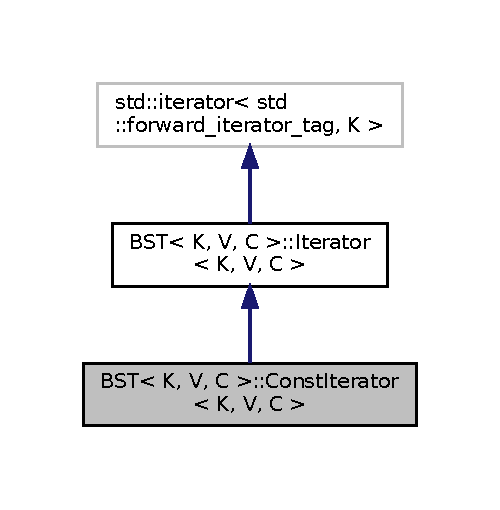
\includegraphics[width=240pt]{classBST_1_1ConstIterator__inherit__graph}
\end{center}
\end{figure}


Collaboration diagram for B\+ST$<$ K, V, C $>$\+:\+:Const\+Iterator$<$ K, V, C $>$\+:
\nopagebreak
\begin{figure}[H]
\begin{center}
\leavevmode
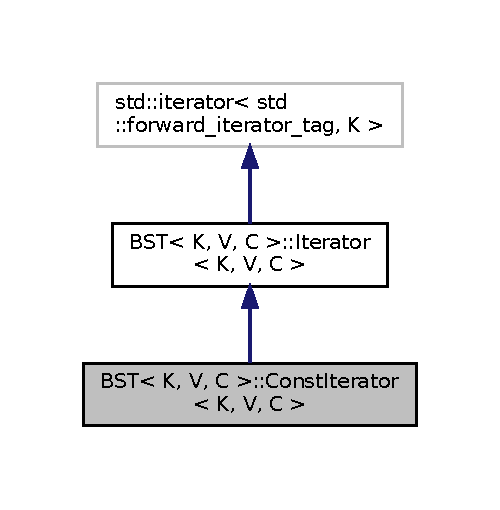
\includegraphics[width=240pt]{classBST_1_1ConstIterator__coll__graph}
\end{center}
\end{figure}
\subsection*{Public Types}
\begin{DoxyCompactItemize}
\item 
\mbox{\Hypertarget{classBST_1_1ConstIterator_a544bf0228b0e126332f80d1d48e1340c}\label{classBST_1_1ConstIterator_a544bf0228b0e126332f80d1d48e1340c}} 
using {\bfseries parent} = \hyperlink{classBST}{B\+ST}$<$ K, V, C $>$\+::\hyperlink{classBST_1_1Iterator}{Iterator}
\end{DoxyCompactItemize}
\subsection*{Public Member Functions}
\begin{DoxyCompactItemize}
\item 
\mbox{\Hypertarget{classBST_1_1ConstIterator_a55a80aeaffdcc3c6614c7a00f6f30bcf}\label{classBST_1_1ConstIterator_a55a80aeaffdcc3c6614c7a00f6f30bcf}} 
const std\+::pair$<$ K, V $>$ \& {\bfseries operator$\ast$} () const
\end{DoxyCompactItemize}


The documentation for this class was generated from the following file\+:\begin{DoxyCompactItemize}
\item 
B\+S\+T.\+cc\end{DoxyCompactItemize}

\hypertarget{classBST_1_1Iterator}{}\section{B\+ST$<$ K, V, C $>$\+:\+:Iterator$<$ K, V, C $>$ Class Template Reference}
\label{classBST_1_1Iterator}\index{B\+S\+T$<$ K, V, C $>$\+::\+Iterator$<$ K, V, C $>$@{B\+S\+T$<$ K, V, C $>$\+::\+Iterator$<$ K, V, C $>$}}


Inheritance diagram for B\+ST$<$ K, V, C $>$\+:\+:Iterator$<$ K, V, C $>$\+:
\nopagebreak
\begin{figure}[H]
\begin{center}
\leavevmode
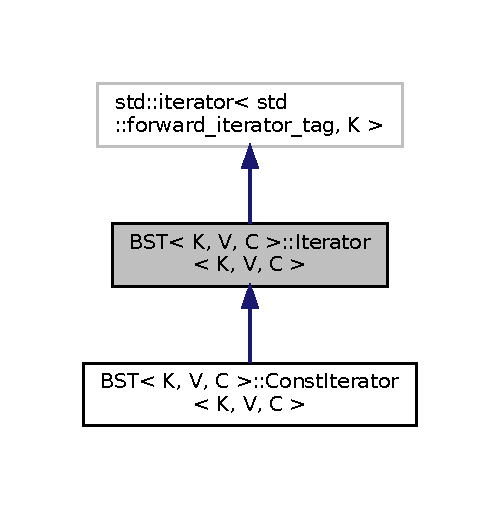
\includegraphics[width=240pt]{classBST_1_1Iterator__inherit__graph}
\end{center}
\end{figure}


Collaboration diagram for B\+ST$<$ K, V, C $>$\+:\+:Iterator$<$ K, V, C $>$\+:
\nopagebreak
\begin{figure}[H]
\begin{center}
\leavevmode
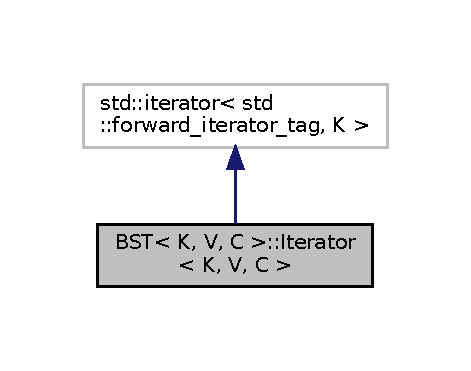
\includegraphics[width=226pt]{classBST_1_1Iterator__coll__graph}
\end{center}
\end{figure}
\subsection*{Public Member Functions}
\begin{DoxyCompactItemize}
\item 
\mbox{\Hypertarget{classBST_1_1Iterator_ad4df476398bc2beefa629a268483b858}\label{classBST_1_1Iterator_ad4df476398bc2beefa629a268483b858}} 
{\bfseries Iterator} (Node $\ast$n)
\item 
\mbox{\Hypertarget{classBST_1_1Iterator_ab63f266d2bb558c16a6b41a37e97b9a7}\label{classBST_1_1Iterator_ab63f266d2bb558c16a6b41a37e97b9a7}} 
{\bfseries Iterator} (const \hyperlink{classBST_1_1Iterator}{Iterator} \&)=default
\item 
\mbox{\Hypertarget{classBST_1_1Iterator_a0fb988985a3cdb4db50669728a2bac38}\label{classBST_1_1Iterator_a0fb988985a3cdb4db50669728a2bac38}} 
std\+::pair$<$ K, V $>$ \& {\bfseries operator$\ast$} () const
\item 
\mbox{\Hypertarget{classBST_1_1Iterator_a32b913d6726c2c4001e0952929aa518b}\label{classBST_1_1Iterator_a32b913d6726c2c4001e0952929aa518b}} 
\hyperlink{classBST_1_1Iterator}{Iterator} \& {\bfseries operator++} ()
\item 
\mbox{\Hypertarget{classBST_1_1Iterator_a8712eb01caaf9e128006f453d5ecd90c}\label{classBST_1_1Iterator_a8712eb01caaf9e128006f453d5ecd90c}} 
bool {\bfseries operator==} (const \hyperlink{classBST_1_1Iterator}{Iterator} \&other)
\item 
\mbox{\Hypertarget{classBST_1_1Iterator_a3a51010bf5571619a28a8d01b243c863}\label{classBST_1_1Iterator_a3a51010bf5571619a28a8d01b243c863}} 
bool {\bfseries operator!=} (const \hyperlink{classBST_1_1Iterator}{Iterator} \&other)
\end{DoxyCompactItemize}


The documentation for this class was generated from the following file\+:\begin{DoxyCompactItemize}
\item 
B\+S\+T.\+cc\end{DoxyCompactItemize}

\chapter{File Documentation}
\hypertarget{BST_8h}{}\section{B\+S\+T.\+h File Reference}
\label{BST_8h}\index{B\+S\+T.\+h@{B\+S\+T.\+h}}


Header file for our Advanced Programming final project.  


{\ttfamily \#include $<$memory$>$}\newline
{\ttfamily \#include $<$utility$>$}\newline
{\ttfamily \#include $<$functional$>$}\newline
{\ttfamily \#include $<$iostream$>$}\newline
{\ttfamily \#include $<$vector$>$}\newline
Include dependency graph for B\+S\+T.\+h\+:
\nopagebreak
\begin{figure}[H]
\begin{center}
\leavevmode
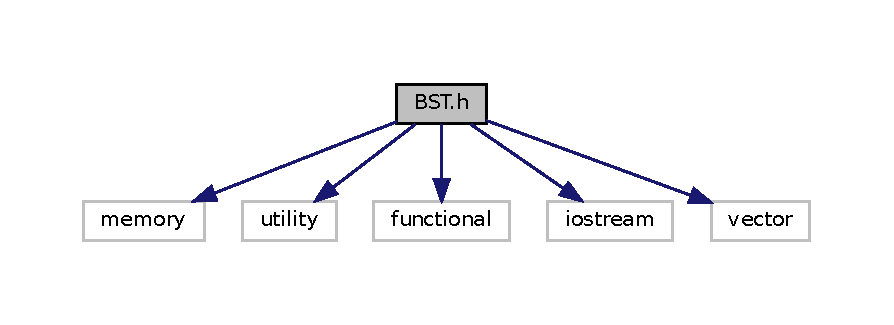
\includegraphics[width=350pt]{BST_8h__incl}
\end{center}
\end{figure}
\subsection*{Classes}
\begin{DoxyCompactItemize}
\item 
class \hyperlink{classBST}{B\+S\+T$<$ K, V, C $>$}
\begin{DoxyCompactList}\small\item\em This class implements a simple Binary Search Tree. \end{DoxyCompactList}\end{DoxyCompactItemize}


\subsection{Detailed Description}
Header file for our Advanced Programming final project. 

\begin{DoxyAuthor}{Author}
Niccolò Rossi, Nicola Meneghini and Lorenzo Fresco 
\end{DoxyAuthor}

%--- End generated contents ---

% Index
\backmatter
\newpage
\phantomsection
\clearemptydoublepage
\addcontentsline{toc}{chapter}{Index}
\printindex

\end{document}
